\input{../../../../.preambles/02-lab_work}
\input{../../../../.preambles/20-math}
\newgeometry{top=1.5cm, bottom=1.5cm, left=1cm, right=1cm}
\begin{document}
    \begin{table}[h!]
        \center
        \begin{tabular}{|C{.5}|C{.2}|C{.25}|} \hline
            \multicolumn{1}{|c|}{\multirow{4}{*}{Лабораторная работа № 605}} &
            Студент, группа & \\ \cline{2-3}
            & Дата выполнения & \\ \cline{2-3}
            & Подпись &  \\ \cline{2-3}
            Определение ширины запрещенной & Дата отчёта & \\ \cline{2-3}
            зоны в кристалле диэлектрика & Оценка &  \\ \cline{2-3}
            & Подпись &  \\ \hline
        \end{tabular}
    \end{table}

    \emph{Цель работы:} изучение закономерностей поглощения света кристаллами с
    точки зрения зонной теории. Определение границы основного поглощения и
    ширины запрещенной зоны кристалла титаната бария.
    
    \emph{Используемые при расчетах формулы:}
    \( \tau = (J - J_T)/(J_0 - J_T); \ \Delta E = hc/\lambda_0 \).

    \begin{figure}[h!]
        \center
        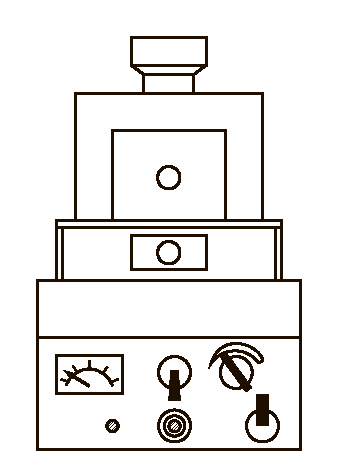
\includegraphics[width=.5\textwidth]{appearance} \\
        \parbox{.5\textwidth}{\caption{Внешний вид установки}}
    \end{figure}
    
    \begin{table}[h!]
        \center \caption{Однократно измеряемые величины и постоянные}
        \begin{tabular}{|*{8}{C{.1}|}} \hline
            \( \phi^* \),~град & \( \phi_{585} \),~град &
                \( \Delta\phi \),~град & \( \lambda_0 \),~нм &
                \( \Delta E \),~Дж & \( \Delta E \),~эВ &
                \( c \),~м/с & \( \hbar \),~Дж\( \cdot \)с \\ \hline
            &&&&&& \( 3 \cdot 10^8 \) &
                \( 1,\!05 \cdot 10^{-34} \) \\ \hline
        \end{tabular}
    \end{table}
    
    \begin{table}[h!]
        \center \caption{Многократно измеряемые величины}
        \begin{tabular}{|*{8}{C{.1}|}} \hline
            \multicolumn{2}{|c|}{Отсчет по} &
                Длина &
                \multicolumn{4}{c|}{Интенсивность света, прошедшего через} &
                Прозрач- \\ \cline{4-7}
            \multicolumn{2}{|c|}{монохроматору, град} &
                волны, нм &
                \multicolumn{2}{c|}{кристалл} &
                \multicolumn{2}{c|}{окно} &
                ность, \% \\ \hline
            \( \phi' \) & \( \phi \) & \( \lambda \) &
                \( J \) & \( J - J_T \) &
                \( J_0 \) & \( J_0 - J_T \) &
                \( \tau \) \\ \hline
            &&&&&&& \\ \hline
            &&&&&&& \\ \hline
            &&&&&&& \\ \hline
            &&&&&&& \\ \hline
            &&&&&&& \\ \hline
            &&&&&&& \\ \hline
            &&&&&&& \\ \hline
            &&&&&&& \\ \hline
            &&&&&&& \\ \hline
            &&&&&&& \\ \hline
            &&&&&&& \\ \hline
            &&&&&&& \\ \hline
            &&&&&&& \\ \hline
        \end{tabular}
    \end{table}
    
    \pagebreak
    
    \subsection{Подсчет погрешности и окончательные результаты}
    \center
    \rule{.95\textwidth}{.5pt} \\ \rule{.95\textwidth}{.5pt}
    \rule{.95\textwidth}{.5pt} \\ \rule{.95\textwidth}{.5pt}
    \rule{.95\textwidth}{.5pt} \\ \rule{.95\textwidth}{.5pt}
    \rule{.95\textwidth}{.5pt} \\ \rule{.95\textwidth}{.5pt}
    \rule{.95\textwidth}{.5pt} \\ \rule{.95\textwidth}{.5pt} \\
    \vspace*{2em}
    
    \emph{Вывод:} \rule{.885\textwidth}{.5pt}
    \rule{.95\textwidth}{.5pt} \\ \rule{.95\textwidth}{.5pt}
    \rule{.95\textwidth}{.5pt}
\end{document}
